\documentclass[a4paper,12pt,titlepage]{article}
\usepackage[utf8]{inputenc}
\usepackage{graphicx} % Required for inserting images
\usepackage[spanish,es-tabla]{babel}
\usepackage[none]{hyphenat}
\usepackage[justification=centering]{caption}
\usepackage{subcaption}
\usepackage{amssymb, amsmath}
\usepackage{gensymb}
\usepackage{fancyhdr}
\usepackage{hyperref}


\lhead{Pequeñas resistencias}
\rhead{Gonzalo Bastos González}

\pagestyle{fancy}

\title{Pequeñas resistencias}
\author{Gonzalo Bastos González}

\begin{document}

\maketitle

\tableofcontents
\newpage

\section{Introducción}

El objetivo de esta práctica es determinar la resistividad de ciertos materiales, que es una magnitud inherente al propio material y está relacionada con su resistencia. Antes que nada debemos señalar la diferencia que existe entre la resistividad y la resistencia. La resistencia se define como la oposición al flujo de corriente eléctrica a través de un conductor, por lo que es una magnitud extensiva, y está relacionada con el voltaje y la intensidad de corriente por la ley de Ohm $(\Delta V = IR)$.

\begin{figure}[h!]
    \begin{subfigure}{0.5\textwidth}
        \centering
        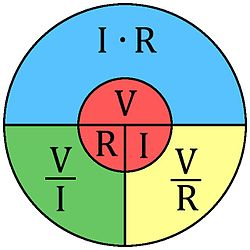
\includegraphics[width=0.5\linewidth]{Images/Ley_de_ohm_-_Organigrama.jpg}
    \end{subfigure}
    \begin{subfigure}{0.42\textwidth}
        \centering
        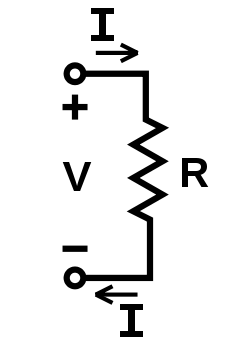
\includegraphics[width=0.5\linewidth]{Images/esquema ohm.png}
    \end{subfigure}
\end{figure}

Por otro lado la resistividad es una magnitud intensiva, depende solo del material y no de su geometría, y se define como la resistencia eléctrica de dicho material. La resistividad y la resistencia del material se relacionan a partir de la siguiente fórmula:

\begin{equation}
    R = \rho \: \frac{L}{S} \Rightarrow \rho = R \: \frac{S}{L}
    \label{Resistividad}
\end{equation}

\begin{itemize}
    \item $R$ es la resistencia del material, en el SI se mide en $\Omega$
    \item $S$ es la sección transversal del material
    \item $L$ es la longitud del material
    \item $\rho$ es la resistividad del material, en el SI se mide en $\Omega \cdot m$
\end{itemize}

Valores altos de resistividad indican que el material es un aislante, mientras que valores bajos indican que el material es un buen conductor. Para hacernos una idea, la resistividad de la mayoría de los metales más comunes, como la plata o el oro es del orden de $10^{-8}\: \Omega \cdot m$, mientras que la resistividad de aislantes como la madera o el vidrio puede llegar a valores del orden de $10^{10}\: \Omega \cdot m$.

\section{Materiales y metodología}

La práctica consta de dos partes bien diferenciadas. En primer lugar determinaremos la resistividad del cobre y del aluminio a partir de dos barras metálicas. En la segunda parte el objetivo será determinar la resistencia entre dos contactos de una caja de conexiones realizando medidas con diferentes cables.

\subsection{Determinación de la resistividad de metales}

Los materiales empleados fueron los siguientes:

\begin{itemize}
    \item Dos barras metálicas de los materiales a estudiar, cobre y aluminio
    \item Generador de corriente continua y cables conductores
    \item Amperímetro y voltímetro
    \item Amplificador de señal
\end{itemize}

El montaje experimental del circuito es el siguiente:

\begin{figure}[h!]
    \begin{subfigure}{0.5\textwidth}
        \centering
        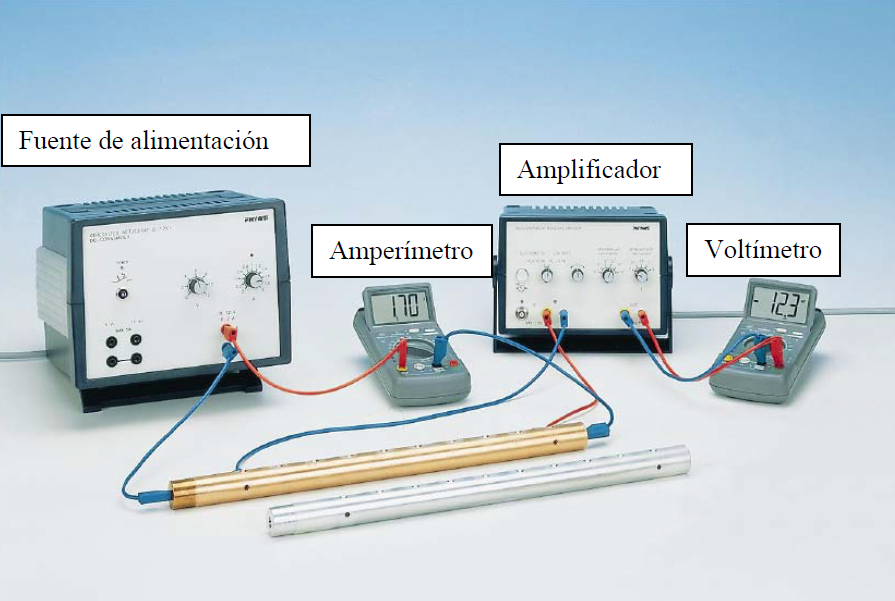
\includegraphics[width=1\linewidth]{Images/montaje experimental.png}
        \subcaption{Material empleado}
    \end{subfigure}
    \begin{subfigure}{0.42\textwidth}
        \centering
        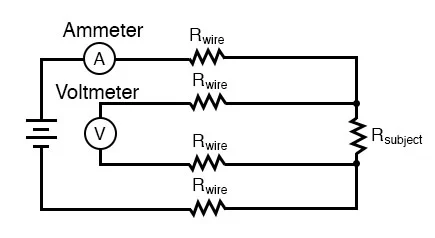
\includegraphics[width=1.5\linewidth]{Images/ohmmeter-example3.png}
        \subcaption{Esquema del circuito}
    \end{subfigure}
    \caption{Montaje experimental}
    \label{Circuito}
\end{figure}



El método utilizado para la medición fue el método de Kelvin o medición a cuatro puntas, como se puede observar en el circuito. En nuestro caso particular el método de la medición a dos puntas, conectando simplemente un óhmetro a cada extremo de la barra, nos proporcionaría un valor lejano al de la resistencia real. Esto se debe a que, pese a ser el método más común, el valor de la resistencia que medimos incluye también la resistencia del cableado, además de la resistencia incógnita. Para resistencias de un valor razonable esta desviación es casi imperceptible, pues la resistencia de los cables es muy baja. No obstante, estamos trabajando con metales conductores que cuentan con una resistencia muy baja, por lo que la interferencia del cableado provocaría que las medidas estuvieran muy lejos de las reales. La ventaja del método de Kelvin es que nos permite medir la resistencia incógnita de forma indirecta a partir de la ley de Ohm, debido a que la intensidad de corriente permanece constante en todo el circuito lo único que necesitamos medir es la caída de potencial entre los contactos de nuestra barra metálica. Además de esto, hay que señalar que, puesto que la resistencia de los voltímetros es muy alta, prácticamente no circula corriente por el circuito interno por lo que la caída de potencial que medimos se puede atribuír totalmente a la barra metálica.

\par Como bien hemos señalado antes, la medida de la resistencia se realizará de forma indirecta a partir de la ley de Ohm. Mediremos 20 pares de valores de intensidad y voltaje distribuidos de forma uniforme entre los $0 \; A$ y los $4 \; A$ que puede suministrar la fuente de alimentación como máximo, separando cada medida por $0,2 \; A$. Para medir el voltaje necesitaremos un amplificador de señal, puesto que la caída de potencial entre los contactos es muy baja. En nuestro caso (Para ambas barras metálicas) el factor de amplificación será de $10^2$, por lo que el resultado medido deberá ser dividido por $100$. Una vez tengamos nuestros $20$ valores de intensidad y voltaje realizaremos un ajuste por mínimos cuadrados para calcular la resistencia.

\par Un último detalle a destacar en la medida de las caídas de potencial (Voltaje) es el efecto del voltaje residual. Como estamos trabajando con un factor de amplificación $100$ la magnitud de la electricidad residual del circuito toma cierta importancia, esto se traduce en que a intensidad cero exista un pequeño voltaje residual que modifica el cero del voltaje. Este efecto debe tenerse en cuenta a la hora de medir la caída de potencial de la barra metálica y puede corregirse de la siguiente forma:

\begin{figure}[h!]
    \centering
    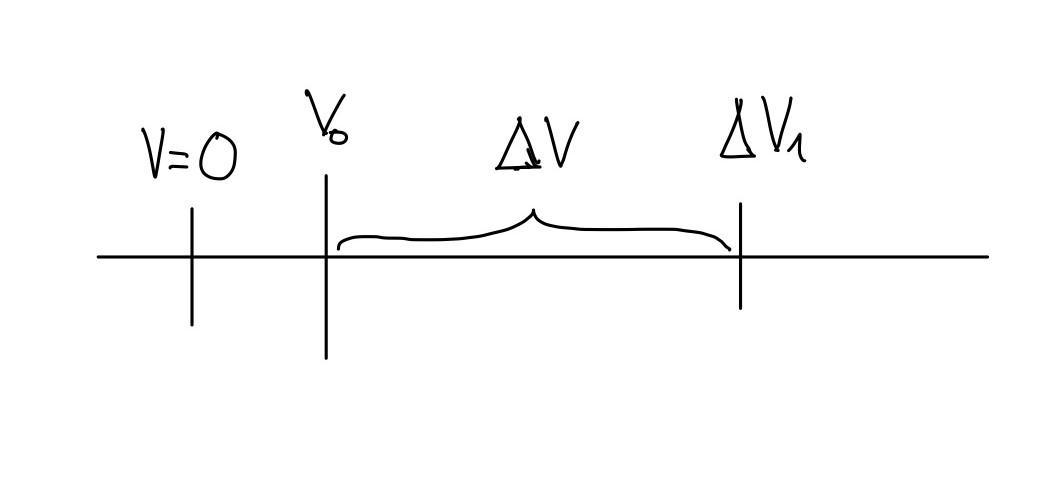
\includegraphics[width=0.65\linewidth]{Images/voltaje residual-4 (002).jpg}
    \caption{Esquema del efecto del voltaje residual}
\end{figure}

\begin{equation}
    \Delta V = \Delta V_{1} - V_{0}
    \label{Voltaje residual}
\end{equation}

Donde $\Delta V$ es la caída de potencial real, $\Delta V_{1}$ es la caída medida y $V_{o}$ es el voltaje residual.

Por tanto, la incertidumbre de la caída de potencial tiene la siguiente expresión:

\begin{equation}
    s(\Delta V) = \sqrt{\left (\frac{\partial \Delta V_{1}}{\partial \Delta V}\right )^2s^2(\Delta V_{1}) + \left (\frac{\partial V_{0}}{\partial \Delta V}\right )^2s^2(V_{o})} = \sqrt{s^2(\Delta V_{1}) + s^2(V_{0})}
    \label{Inc Voltaje residual}
\end{equation}

Como la incertidumbre de todos los voltajes medidos es la misma, podemos expresar la incertidumbre de la caída de potencial real de la siguiente forma:

\begin{equation}
    s(\Delta V) = \sqrt{2}\cdot s(\Delta V_{1})
    \label{Inc voltaje}
\end{equation}

\par Una vez conocido el valor de la resistencia de la barra metálica podemos determinar su resistividad a partir de la Ec.\ref{Resistividad}, midiendo la distancia entre contactos y la sección transversal. Además de eso, calcularemos la incertidumbre de la resistividad a partir de propagación de incertidumbres de la siguiente forma:

\begin{align}
    s(\rho) &= \sqrt{\left (\frac{\partial \rho}{\partial R}\right )^2s^2(R)  +  \left (\frac{\partial \rho}{\partial L}\right )^2s^2(L)  +  \left (\frac{\partial \rho}{\partial S}\right )^2s^2(S)} \nonumber \\
    s(\rho) &= \sqrt{\left (\frac{S}{L}\right )^2s^2(R)  +  \left (\frac{-RS}{L^2}\right )^2s^2(L)  +  \left (\frac{R}{L}\right )^2s^2(S)}
    \label{Inc resistividad}
\end{align}

El valor de la sección transversal se obtiene midiendo el radio y calculando el área del círculo por lo que su incertidumbre es la siguiente:

\begin{align}
    \begin{split}
    S &= \pi r^2 \\
    s(S) = \sqrt{\left (\frac{\partial S}{\partial r}\right )^2s^2(S)} &= 2\pi r s(r)
    \end{split}
    \label{Inc sección}
\end{align}

\newpage

Las incertidumbres del diámetro de la barra metálica y de la distancia entre contactos vienen dadas por el aparato de medida, la regla, que contaba con una incertidumbre de $0,5 \; mm = 0,0005 \; m$. Por tanto, la incertidumbre del radio será la mitad de la del diámetro.

\begin{align}
    \begin{split}
        s(r) &=\frac{s(d)}{2}= 0,00025 m  \\
        s(L) &= 0,0005 m
    \end{split}
\end{align}

Por último, cabe destacar que ciertos valores de voltaje medidos son el valor medio entre los límites de oscilación del voltímetro, pues la amplifiación provocaba cierta oscilación en el voltaje. No obstante, para realizar el tratamiento de datos hemos considerado tomar todos los valores con una incertidumbre constante, el doble de la dada por el voltímetro. La justificación para hacer esto es que las oscilaciones no provocaban cambios excesivos en el valor y este terminaba por estabilizarse entorno a un voltaje determinado. Por tanto, todos los ajustes por mínimos cuadrados realizados fueron regresiones lineales simples sin término independiente y las ecuaciones empleadas fueron las siguientes:

\begin{equation}
    b=\frac{\sum_{i}x_{i}y_{i}}{\sum_{i}x_{i}^2}
\end{equation}
\begin{equation}
    s=\sqrt{\frac{\sum_{i}(y_{i}-bx_{i})^2}{n-1}}
\end{equation}
\begin{equation}
    s(b)=\frac{s}{\sqrt{\sum_{i}x_{i}^2}}
\end{equation}
\begin{equation}
    r=\frac{\sum_{i}x_{i}y_{i}}{\sqrt{(\sum_{i}x_{i}^2)(\sum_{i}y_{i}^2)}}
\end{equation}

\newpage

\subsection{Determinación de la resistencia entre contactos de la caja de conexiones}

Los materiales empleados fueron los siguientes:

\begin{itemize}
    \item Caja de conexiones
    \item Generador de corriente continua y cableado
    \item Tres cables conductores de diferentes longitudes: 2000 mm, 600 mm, 100 mm
    \item Amperímetro y voltímetro
\end{itemize}

El esquema del montaje experimental es el siguiente:

\begin{figure}[h!]
    \centering
    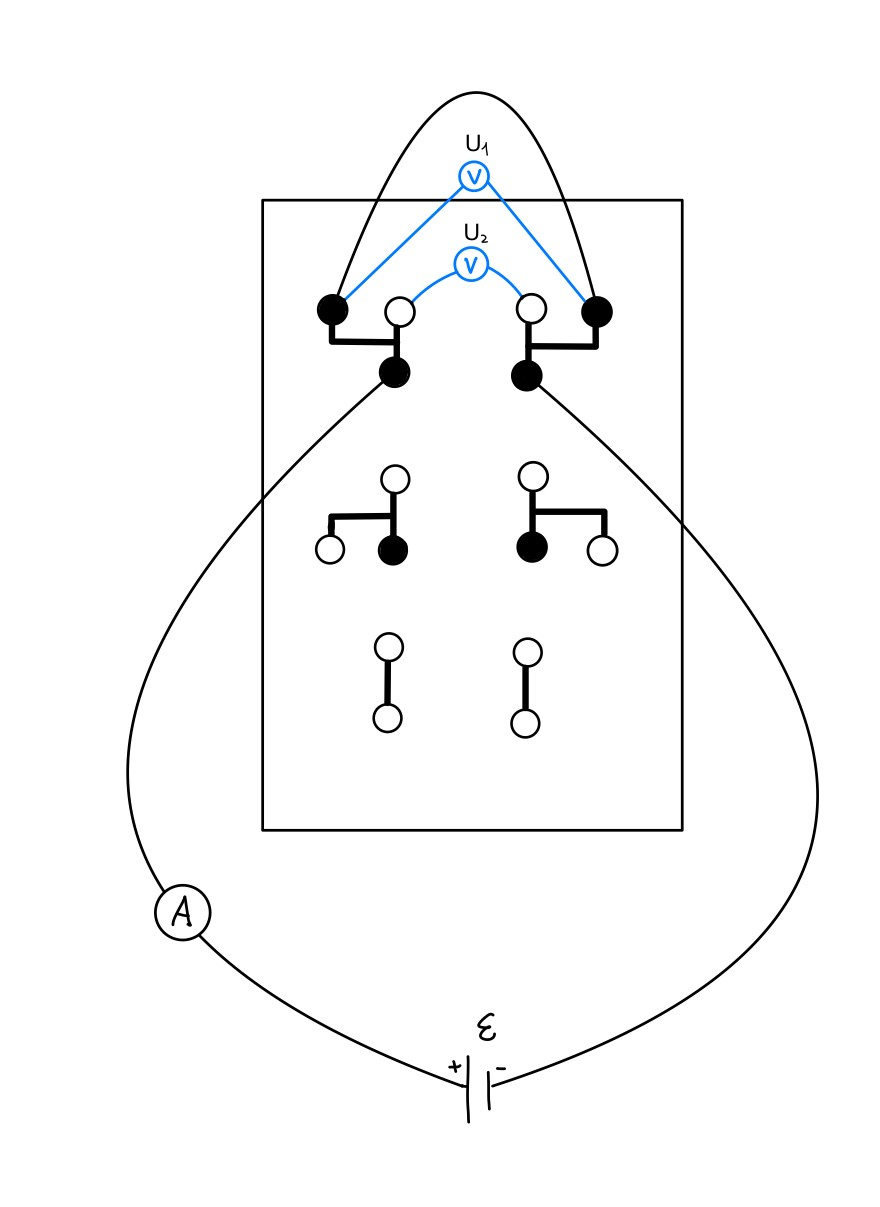
\includegraphics[width=0.65\linewidth]{Images/esquema caja conexiones.jpeg}
    \caption{Esquema del circuito experimental}
    \label{Caja de conexiones}
\end{figure}

En el esquema podemos observar dos posibles configuraciones del voltímetro, $U_{1}$ y $U_{2}$. En la configuración $U_{1}$ conectamos el voltímetro directamente al cable, por lo que la caída de potencial medida se debe únicamente a los diferentes cables conductores. Por otra parte, en la configuración $U_{2}$ conectamos el voltímetro a los contactos libres, por lo que la caída de potencial medida se debe al cableado y a los contactos entre los conductores.

\par Las medidas se realizarán de forma idéntica a las realizadas en el apartado anterior, mediremos los valores de voltaje provocados por diferentes intensidades distribuidas uniformemente en el rango de $0$ a $4 \;A$. A diferencia del apartado anterior, estas medidas fueron tomadas sin amplificación, pues los intentos de trabajar con factores de amplificación de 100 e incluso 10 provocaban oscilaciones muy importantes en la medida. Respecto a las medidas debemos destacar también que en los casos de los cables más largos no fuimos capaces de llegar a los $4 \: A$ de intensidad, pues a partir de valores del orden de $3\; A$ las medidas comenzaban a oscilar y perdían la linealidad.

\par Una vez tengamos los valores de intensidad y voltaje calcularemos la resistencia por un ajuste de mínimos cuadrados en cada caso. La forma de determinar la resistencia entre contactos de la caja de conexiones es la siguiente:

\begin{equation}
    R_{C} = \frac{R_{2}-R_{1}}{2}
    \label{Resistencia contactos}
\end{equation}

La resistencia entre contactos se calcula restando a la resitencia total la resistencia del cable y dividiendo entre dos, para calcular la resistencia solo entre los contactos de un lado. La incertidumbre asociada es la siguiente:

\begin{equation}
    s(R_{C}) = \sqrt{\left (\frac{\partial R_{C}}{\partial R_{2}}\right )^2s^2(R_{2})  +  \left (\frac{\partial R_{C}}{\partial R_{1}}\right )^2s^2(R_{1})} = \frac{1}{2}\sqrt{s^2(R_{2})  +  s^2(R_{1})}
    \label{Inc Resistencia caja}
\end{equation}

Obtendremos 3 valores de $R_{C}$ para cada uno de los tres cables (100 mm, 600 mm y 2000 mm) con los cuales podremos determinar el valor de la resistencia entre contactos calculando su media aritmética.

\newpage

\section{Análisis de datos}

\subsection{Resistividad del cobre}

Como se ha detallado en la metodología, tomamos 20 valores de intensidad y voltaje, que serán representados en una tabla a continuación.

\par La incertidumbre de la intensidad viene dada por la fuente de alimentación:

\begin{equation}
    s(I) = 0,01 \; A
\end{equation}

La incertidumbre del voltaje medido, como hemos explicado antes, debe tener en cuenta el factor de amplificación y además la escala del voltímetro, que para estas medidas estaba en $mV$. Por tanto, teniendo en cuenta que trabajamos con un factor de amplificación 100 debemos dividir todos los resultados entre $10^5$ para obtener los valores en unidades del SI. La incertidumbre del voltímetro era de $0,1 \; mV$, por tanto la incertidumbre de nuestras medidas fue de:

\begin{equation}
    s(\Delta V_{1}) = 2 \cdot 10^{-6}\; V
\end{equation}

Debemos tener en cuenta el valor del voltaje residual, que afectará a nuestra incertidumbre, como hemos mencionado anteriormente, por lo que el valor final de la incertidumbre de las caídas de potencial es:

\begin{equation}
    s(\Delta V) = \sqrt{2}\cdot s(\Delta V_{1}) = 2,8 \cdot 10^{-6} \; V
\end{equation}



\bigskip

\begin{table}[h!]
    \centering
    \begin{tabular}{|c|c|c|c|}
        \hline Intensidad($A$) & Voltaje($mV$) & Intensidad($A$) & Voltaje($mV$) \\
        \hline
        $0,2$ & $0,005$ & $2,2$ & $0,028$\\
        \hline
        $0,4$ & $0,007$ & $2,4$ & $0,030$  \\
        \hline
        $0,6$ & $0,009$ & $2,6$ & $0,032$  \\
        \hline
        $0,8$ & $0,013$ & $2,8$ & $0,034$  \\
        \hline
        $1,0$ & $0,015$ & $3,0$ & $0,036$  \\
        \hline
        $1,2$ & $0,016$ & $3,2$ & $0,038$  \\
        \hline
        $1,4$ & $0,018$ & $3,4$ & $0,041$  \\
        \hline
        $1,6$ & $0,020$ & $3,6$ & $0,043$  \\
        \hline
        $1,8$ & $0,023$ & $3,8$ & $0,046$  \\
        \hline
        $2,0$ & $0,026$ & $4,0$ & $0,048$  \\
        \hline
    \end{tabular}
    \caption{Medidas de la barra de cobre}
\end{table}

Los datos medidos están expresados en $mV$ y quitando ya el efecto de la amplificación y del voltaje residual (Ec.\ref{Voltaje residual}, donde el valor del cero resultó ser de $14,8 \; mV$), para trabajar con las caídas de potencial reales.

\par A partir de estos datos vamos a hacer una regresión lineal simple sin término independiente por el método de los mínimos cuadrados para aproximar nuestros puntos experimentales a una recta del tipo $y=bx$ usando las Ec.8, Ec.9, Ec.10 y Ec.11. La variable dependiente ($y$) será la intensidad y la variable dependiente ($x$) será el voltaje. Los valores obtenidos fueron:

\begin{equation}
    \begin{gathered}
        b = 1.226 \cdot 10^{-5}\; \Omega
        \\
        s(b) = 1.4 \cdot 10^{-7}\; \Omega
        \\
        r = 0.998
        \\
        s = 1.5 \cdot 10^{-6}
    \end{gathered}
\end{equation}

Por tanto la recta a la que aproximamos nuestros puntos tiene la siguiente ecuación:

\begin{equation}
    y = 1,226 \cdot 10^{-5}x
\end{equation}

Donde la pendiente de la recta, haciendo una similitud de la ley de Ohm ($V=IR$), resulta ser la resistencia de la barra de cobre $(1,226 \cdot 10^{-5}\;  \Omega)$.

\begin{figure}[h!]
    \centering
    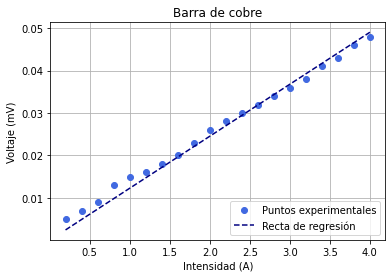
\includegraphics[width=0.85\linewidth]{Images/plotCobre.png}
    \caption{Datos experimentales y recta de regresión de la barra de cobre}
\end{figure}

\newpage

\par A partir del valor de la resistencia de la barra y de los datos de su geometría podemos calcular el valor de la resistividad del cobre a partir de la Ec.\ref{Resistividad}.

\par Los valores medidos de la distancia entre contactos y radio son:

\begin{align}
    \begin{split}
        r &= 0,0125\; m\\
        L &= 0,325\; m
    \end{split}
\end{align}

Entonces su sección transversal es:

\begin{equation}
    S = \pi r^2 = 4,9 \cdot 10^{-4}\; m^2
\end{equation}

\begin{equation}
    \rho_{Cu} = R \: \frac{S}{L} = 1.851 \cdot 10^{-8} \; \Omega \cdot m
\end{equation}

Las incertidumbres asociadas, calculadas a partir de las Ec.\ref{Inc resistividad} y Ec.\ref{Inc sección}, son:

\begin{equation}
    \begin{gathered}
        s(S) = 2\pi r s(r) = 2,0 \cdot 10^{-5} \; m^2
        \\
        s(\rho_{Cu}) = 7.7 \cdot 10^{-10} \; \Omega \cdot m
    \end{gathered}
\end{equation}

Por tanto, el valor final de la resistividad del cobre es de:

\begin{equation}
    \rho_{Cu} = 1.851 \cdot 10^{-8} \pm 7.7 \cdot 10^{-10} \; \Omega \cdot m
\end{equation}

El valor real de la resistividad del cobre es de $1,678 \cdot 10^{-8} \Omega \cdot m$, que aunque no entra en el rango de incertidumbre se encuentra muy cerca del valor experimental.

\subsection{Resistividad del aluminio}

El procedimiento para determinar la resistividad del aluminio es exactamente idéntico, tomaremos los 20 valores de voltaje e intensidad y después realizaremos un ajuste por el método de los mínimos cuadrados para calcular la resistencia de la barra de aluminio valiéndonos de la ley de Ohm. Como el factor de amplificación es el mismo y los aparatos de medida trabajan con la misma escala las incertidumbres en los valores de las caídas de potencial e intensidades no cambian.

\begin{equation}
    \begin{gathered}
    s(I) = 0,01 \; A\\    
    s(\Delta V) = 2,8 \cdot 10^{-6} \; V
    \end{gathered}
\end{equation}

Los valores medidos fueron los siguientes (Expresados sin amplificación):

\begin{table}[h!]
    \centering
    \begin{tabular}{|c|c|c|c|}
        \hline
        Intensidad (A) & Voltaje (mV) & Intensidad (A) & Voltaje (mV) \\
        \hline
        $0,2$ & $0,002$ & $2,2$ & $0,039$ \\
        \hline
        $0,4$ & $0,005$ & $2,4$ & $0,041$ \\
        \hline
        $0,6$ & $0,010$ & $2,6$ & $0,045$ \\
        \hline
        $0,8$ & $0,015$ & $2,8$ & $0,048$ \\
        \hline
        $1,0$ & $0,017$ & $3,0$ & $0,051$ \\
        \hline
        $1,2$ & $0,020$ & $3,2$ & $0,054$ \\
        \hline
        $1,4$ & $0,023$ & $3,4$ & $0,058$ \\
        \hline
        $1,6$ & $0,028$ & $3,6$ & $0,061$ \\
        \hline
        $1,8$ & $0,031$ & $3,8$ & $0,065$ \\
        \hline
        $2,0$ & $0,035$ & $4,0$ & $0,069$ \\
        \hline
    \end{tabular}
    \caption{Datos experimentales de la barra de aluminio}
\end{table}

Los datos serán ajustados a una recta del tipo $y=bx$ por un ajuste de mínimos cuadrados igual que en apartado anterior, donde $b$ representa la resistencia. Los valores obtenidos fueron:

\begin{equation}
    \begin{gathered}
        b = R = 1.7120 \cdot 10^{-5} \; \Omega \\
        s(b) = s(R) = 7,7 \cdot 10^{-8} \; \Omega\\
        r = 0,9998 \\
        s = 8,3\cdot 10^{-7}
    \end{gathered}
\end{equation}

Por tanto, la recta de regresión a la que vamos a aproximar nuestros puntos experimentales es la siguiente:

\begin{equation}
    y = 1.226 \cdot 10^{-5}x
\end{equation}

\begin{figure}[h!]
    \centering
    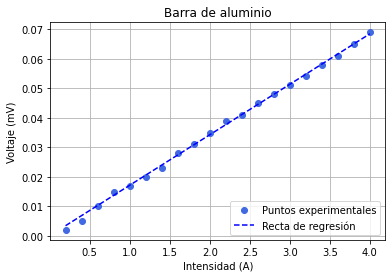
\includegraphics[width=0.85\linewidth]{Images/plotAluminio.png}
    \caption{Datos experimentales y recta de regresión de la barra de aluminio}
\end{figure}

\newpage

Las dimensiones de la barra son las misma, tanto en radio como en distancia entre contactos, por lo que las incertidumbres se mantienen:

\begin{equation}
    \begin{gathered}
        s(S) = 2,0\cdot 10^{-5} \; m^2 \\
        s(L) = 0,0005m
    \end{gathered}
\end{equation}

El valor de la resistencia de la barra es:

\begin{equation}
    R = 1.226 \cdot 10^{-5} \pm 1.4 \cdot 10^{-7} \; \Omega
\end{equation}

Aplicando la Ec.\ref{Resistividad} y la Ec.\ref{Inc resistividad} el valor de la resistividad del aluminio y su incertidumbre es de:

\begin{equation}
    \rho_{Al} = 2.58 \cdot 10^{-8} \pm
    1.0\cdot 10^{-9} \; \Omega \cdot m
\end{equation}

El valor real de la resistividad del aluminio es de $2,650 \cdot 10^{-8} \; \Omega \cdot m$, por lo que nuestro resultado se ajusta en gran medida a la realidad.

\newpage

\subsection{Determinación de la resistencia entre contactos de la caja de conexiones}

Como hemos mencionado en la metodología para la determinación de la resistencia entre contactos vamos a medir la resistencia por dos caminos ($U_{1}$ y $U_{2}$), de forma que a partir de la Ec.\ref{Resistencia contactos} podremos calcular la resistencia entre contactos. Las medidas se realizarán igual que en las barras metálicas, 20 pares de valores (En algunos casos menos por problemas técnicos) de intensidad y voltaje para los caminos $U_{1}$ y $U_{2}$ con tres cables de longitud diferente. A partir de ahí obtendremos tres valores de la resistencia entre contactos que deberemos comparar.

\subsubsection{Cable de 100 mm}

Los valores de intensidad y voltaje medidos para el segmento $U_{1}$, formado solo por el cable, son los siguientes:

\begin{table}[h!]
\centering
    \begin{tabular}{|c|c|c|c|}
        \hline
        Intensidad (A) & Voltaje (mV) & Intensidad (A) & Voltaje (mV) \\ \hline
        $0,2$ & $1,61$ & $2,2$ & $20,0$ \\ \hline
        $0,4$ & $3,5$ & $2,4$ & $21,5$ \\ \hline
        $0,6$ & $5,3$ & $2,6$ & $23,2$ \\ \hline
        $0,8$ & $7,1$ & $2,8$ & $25,6$ \\ \hline
        $1,0$ & $8,9$ & $3,0$ & $27,2$ \\ \hline
        $1,2$ & $10,9$ & $3,2$ & $29,2$ \\ \hline
        $1,4$ & $13,0$ & $3,4$ & $30,7$ \\ \hline
        $1,6$ & $14,6$ & $3,6$ & $32,6$ \\ \hline
        $1,8$ & $16,5$ & $3,8$ & $34,9$ \\ \hline
        $2,0$ & $18,1$ & $4,0$ & $35,7$ \\ \hline
    \end{tabular}
    \caption{Datos experimentales del cable de 100 mm}
\end{table}

A partir de estos datos vamos a realizar un ajuste por el método de los mínimos cuadrados donde ajustaremos nuestros datos experimentales a una recta del tipo $y=bx$. Haciendo una similitud con la ley de Ohm $(V=IR)$, la pendiente de la recta será la resistencia del cable. Los parámetros obtenidos fueron los siguientes:

\begin{equation}
    \begin{gathered}
        b =R_{1}= 0.009058 \; \Omega 
        \\
        s(b) = s(R_{1})= 2.2 \cdot 10^{-5} \; \Omega
        \\
        r = 0.99994
        \\
        s = 0.00024
    \end{gathered}
\end{equation}

Por tanto la recta a la que aproximaremos nuestros puntos es:

\begin{equation}
    y = 0,009058x
\end{equation}

Los valores obtenidos para el segmento $U_{2}$, formado por el cable y la caja de conexiones, son los siguientes:

\begin{table}[h!]
    \centering
    \begin{tabular}{|c|c|c|c|}
        \hline
        Intensidad (A) & Voltaje (mV) & Intensidad (A) & Voltaje (mV) \\
        \hline
        $0,2$ & $4,2$ & $2,2$ & $47,6$ \\
        \hline
        $0,4$ & $8,6$ & $2,4$ & $51,9$ \\
        \hline
        $0,6$ & $12,9$ & $2,6$ & $56,2$ \\ 
        \hline
        $0,8$ & $17,2$ & $2,8$ & $60,5$ \\
        \hline
        $1,0$ & $21,5$ & $3,0$ & $64,4$ \\
        \hline
        $1,2$ & $25,9$ & $3,2$ & $68,7$ \\
        \hline
        $1,4$ & $30,1$ & $3,4$ & $73,0$ \\ 
        \hline
        $1,6$ & $34,8$ & $3,6$ & $77,3$ \\
        \hline
        $1,8$ & $39,0$ & $3,8$ & $81,5$ \\
        \hline
        $2,0$ & $43,3$ & $4,0$ & $85,8$ \\ 
        \hline
    \end{tabular}
    \caption{Datos experimentales del cable de 100 mm y la caja de conexiones}
\end{table}

A partir de estos datos vamos a realizar un ajuste por el método de los mínimos cuadrados donde ajustaremos nuestros datos experimentales a una recta del tipo $y=bx$. Haciendo una similitud con la ley de Ohm $(V=IR)$, la pendiente de la recta será la resistencia del cable. Los parámetros obtenidos fueron los siguientes:

\begin{equation}
    \begin{gathered}
        b = R_{2} =0,021517 \; \Omega 
        \\
        s(b) =s(R_{2})= 1,9 \cdot 10^{-5} \; \Omega
        \\
        r = 0,999992
        \\
        s = 0,00020
    \end{gathered}
\end{equation}

Por tanto la recta a la que aproximaremos nuestros puntos es:

\begin{equation}
    y = 0,021517x
\end{equation}

Cabe destacar que en los valores de caída de potencial reflejados en las tablas ya hemos tenido en cuenta el valor del voltaje residual, que situaba al cero en un valor de $0,4 \; mV$. Para corregir este efecto aplicamos la Ec.\ref{Voltaje residual} y restamos el valor del cero residual a todos los valores medidos. Esta correción afecta a la incertidumbre y tendremos que aplicar la Ec.\ref{Inc voltaje}.

\newpage

\par A diferencia de los apartados anteriores, al no estar trabajando con el amplificador, los valores medidos en el voltímetro no oscilaban, por lo que hemos considerado la incertidumbre del propio voltímetro $(0,1 \; mV=10 \cdot 10^{-4} \; V)$ como la incertidumbre de las caídas de potencial medidas.

\begin{equation}
    s(\Delta V) = \sqrt{2}\cdot 10^{-4} \; V
\end{equation}

La incertidumbre de la intensidades la misma, pues depende solo de la fuente de alimentación:

\begin{equation}
    s(I) = 0,01 \; A
\end{equation}

Finalmente, en la siguiente figura podremos ver la representación gráfica de nuestros ajustes:

\begin{figure}[h!]
    \centering
    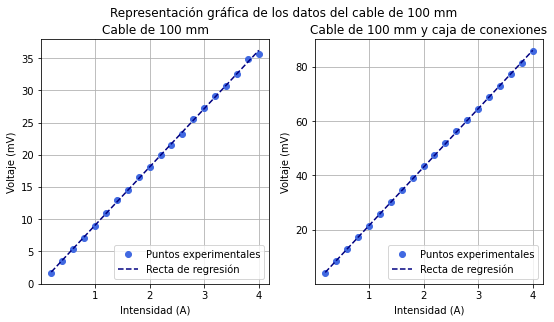
\includegraphics[width=0.9\linewidth]{Images/plotCable1.png}
    \caption{Representación gráfica de los datos experimentales del cable de 100 mm}
\end{figure}

A partir de los ajustes podemos calcular la resistencia entre contactos de la caja de conexiones y su incertidumbre usando la Ec.\ref{Resistencia contactos} y la Ec.\ref{Inc Resistencia caja}:

\begin{equation}
    \begin{gathered}
        R_{C1} = 0.006230 \; \Omega\\
        s(R_{C1}) = 1.5 \cdot 10^{-5} \Omega
    \end{gathered}
\end{equation}

\newpage

\subsubsection{Cable de 600 mm}

El procedimiento será el mismo que para el cable de 100 mm, en primer lugar tomaremos 20 valores de intensidad y voltaje. A diferencia del apartado anterior no había voltaje residual a la hora de realizar las medidas por lo que la incertidumbre del voltaje será menor y será la del propio voltímetro, pues tampoco había oscilaciones en el valor medido. La incertidumbre de la intensidad es la misma.

\begin{equation}
    \begin{gathered}
        s(\Delta V) = 10^{-4} \; V \\
        s(I) = 0,01\; A
    \end{gathered}
\end{equation}

Los valores medidos para el segmento $U_{1}$, formado solo por el cable, fueron los siguientes:

\begin{table}[h!]
    \centering
    \begin{tabular}{|c|c|c|c|}
        \hline
        Intensidad (A) & Voltaje (mV) & Intensidad (A) & Voltaje (mV) \\
        \hline
        $0,2$ & $4,2$ & $2,2$ & $47,4$ \\
        \hline
        $0,4$ & $8,5$ & $2,4$ & $51,7$ \\
        \hline
        $0,6$ & $12,8$ & $2,6$ & $56,1$ \\
        \hline
        $0,8$ & $17,1$ & $2,8$ & $60,4$ \\
        \hline
        $1,0$ & $21,4$ & $3,0$ & $64,8$ \\
        \hline
        $1,2$ & $25,8$ & $3,2$ & $69,2$ \\
        \hline
        $1,4$ & $30,1$ & $3,4$ & $73,6$ \\
        \hline
        $1,6$ & $34,4$ & $3,6$ & $77,9$ \\
        \hline
        $1,8$ & $38,7$ & $3,8$ & $82,4$ \\
        \hline
        $2,0$ & $43,0$ & $4,0$ & $86,8$ \\
        \hline
    \end{tabular}
    \caption{Datos experimentales del cable de 600 mm (Segemto $U_{1}$)}
\end{table}

A partir de estos datos vamos a realizar un ajuste por el método de los mínimos cuadrados donde ajustaremos nuestros datos experimentales a una recta del tipo $y = bx$. Haciendo una similitud con la ley de Ohm (V = IR), la pendiente de la recta será la resistencia del cable. Los parámetros obtenidos fueron los siguientes:

\begin{equation}
    \begin{gathered}
        b = R_{1}=  0.021611 \; \Omega
        s(b)= s(R_{1}) = 1.7 \cdot 10^{-5} \; \Omega
        r =  0.999994
        s =  0.00018
    \end{gathered}
\end{equation}

Por tanto la recta a la que aproximamos nuestros datos es:

\begin{equation}
    y = 0.021611x
\end{equation}

Para el segmento $U_{2}$, formado por el cable de 600 mm y la caja de conexiones, hay que señalar que , como mencionamos en la metodología, a partir de ciertos valores de intensidad los voltajes medidos comenzaron a oscilar y perder la linealidad. Por este motivo nuestras medidas solo llegan a los $3,4$ A de intensidad. Los valores obtenidos fueron los siguientes:

\begin{table}[h!]
    \centering
    \begin{tabular}{|c|c|c|c|}
        \hline
        Intensidad (A) & Voltaje (mV) & Intensidad (A) & Voltaje (mV) \\
        \hline
        $0,2$ & $11,4$ & $2,0$ & $113,3$ \\
        \hline
        $0,4$ & $22,8$ & $2,2$ & $124,5$ \\
        \hline
        $0,6$ & $34,0$ & $2,4$ & $135,6$ \\
        \hline
        $0,8$ & $45,4$ & $2,6$ & $146,7$ \\
        \hline
        $1,0$ & $56,7$ & $2,8$ & $157,9$ \\
        \hline
        $1,2$ & $68,1$ & $3,0$ & $169,1$ \\
        \hline
        $1,4$ & $79,4$ & $3,2$ & $180,3$ \\
        \hline
        $1,6$ & $90,7$ & $3,4$ & $191,4$ \\
        \hline
        $1,8$ & $102$ &  &  \\
        \hline
    \end{tabular}
    \caption{Datos expeerimentales del cable de 600 mm y la caja de conexiones}
\end{table}

A partir de estos datos vamos a realizar un ajuste por el método de los mínimos cuadrados donde ajustaremos nuestros datos experimentales a una recta del tipo $y = bx$. Haciendo una similitud con la ley de Ohm (V = IR), la pendiente de la recta será la resistencia del cable. Los parámetros obtenidos fueron los siguientes:

\begin{equation}
    \begin{gathered}
        b = R_{2} = 0,056455 \; \Omega \\
        s(b) = s(R_{2}) = 3.6 \cdot 10^{-5} \; \Omega \\
        r =  0.999996 \\
        s =  0.00031
    \end{gathered}
\end{equation}

Por tanto la recta a la que aproximamos nuestros datos es:

\begin{equation}
    y = 0,056455x
\end{equation}

En la siguiente figura podemos ver una representación gráfica de nuestros datos experimentales y el resultado del ajuste:

\begin{figure}[h!]
    \centering
    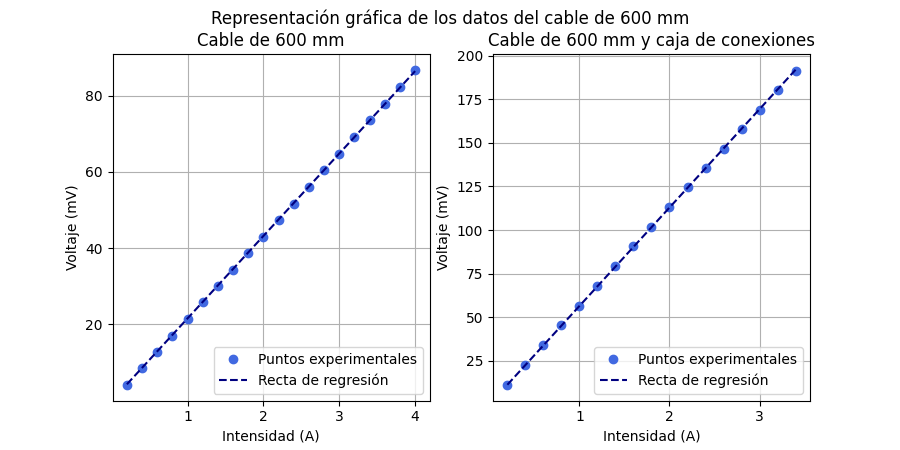
\includegraphics[width=0.95\linewidth]{Images/plotCable2.png}
    \caption{Datos experimentales y rectas de rgresión del cable de 600 mm}
\end{figure}

\newpage

A partir de los ajustes podemos calcular la resistencia entre contactos de la caja de conexiones y su incertidumbre usando la Ec.\ref{Resistencia contactos} y la Ec.\ref{Inc Resistencia caja}:

\begin{equation}
    \begin{gathered}
        R_{C2} = 0.017422 \; \Omega\\
        s(R_{C2}) = 2.6 \cdot 10^{-5}\; \Omega
    \end{gathered}
\end{equation}



\subsubsection{Cable de 2000 mm}

El procedimiento será el mismo que para los otros dos cables, en primer lugar tomaremos 20 valores de intensidad y voltaje. A diferencia del apartado anterior no había voltaje residual a la hora de realizar las medidas por lo que la incertidumbre del voltaje será la del propio voltímetro, pues tampoco había oscilaciones en el valor medido. No obstante los valores de la caída de potencial medidos se pasaban del límite de la escala de 200 mV con la que trabajamos durante toda la práctica, por lo que tuvimos que aumentar la escala y con ello aumenta la incertidumbre. La incertidumbre de la intensidad es la misma.

\begin{equation}
    \begin{gathered}
        s(\Delta V) = 10^{-3} \; V \\
        s(I) = 0,01\; A
    \end{gathered}
\end{equation}

A la hora de realizar las medidas nos encontramos, de la misma forma que en el apartado anterior, que a voltajes altos las medidas comenzaron a oscilar y perdían la linealidad, por lo que realizamos menos medidas. Los valores medidos para el segmento $U_{1}$, formado solo por el cable, fueron los siguientes:

\begin{table}[h!]
    \centering
    \begin{tabular}{|c|c|c|c|}
        \hline
        Intensidad (A) & Voltaje (V) & Intensidad (A) & Voltaje (V) \\ \hline
        $0,2$ & $0,029$ & $1,8$ & $0,302$ \\ \hline
        $0,4$ & $0,061$ & $2,0$ & $0,337$ \\ \hline
        $0,6$ & $0,093$ & $2,2$ & $0,372$ \\ \hline
        $0,8$ & $0,127$ & $2,4$ & $0,407$ \\ \hline
        $1,0$ & $0,163$ & $2,6$ & $0,452$ \\ \hline
        $1,2$ & $0,196$ & $2,8$ & $0,489$ \\ \hline
        $1,4$ & $0,233$ & $3,0$ & $0,525$ \\ \hline
        $1,6$ & $0,267$ & $3,2$ & $0,570$ \\ \hline
    \end{tabular}
    \caption{Datos experimentales del cable de 2000 mm}
\end{table}

A partir de estos datos vamos a realizar un ajuste por el método de los mínimos cuadrados donde ajustaremos nuestros datos experimentales a una recta del tipo $y = bx$. Haciendo una similitud con la ley de Ohm (V = IR), la pendiente de la recta será la resistencia del cable. Los parámetros obtenidos fueron los siguientes:

\begin{equation}
    \begin{gathered}
        b = R_{1} = 0.1720 \; \Omega \\
        s(b) = s(R_{1}) = 0.0012\; \Omega \\
        r =  0.9996 \\
        s =  0.0095
    \end{gathered}
\end{equation}

Por tanto la recta a la que aproximamos nuestros datos es:

\begin{equation}
    y = 0.1720x
\end{equation}

Para el segmento $U_{2}$, formado por el cable de 2000 mm y la caja de conexiones, hay que señalar que , como mencionamos en la metodología, a partir de ciertos valores de intensidad los voltajes medidos comenzaron a oscilar y perder la linealidad. Por este motivo nuestras medidas solo llegan a los $3$ A de intensidad. Los valores obtenidos fueron los siguientes:

\begin{table}[h!]
    \centering
    \begin{tabular}{|c|c|c|c|}
        \hline
        Intensidad (A) & Voltaje (V) & Intensidad (A) & Voltaje (V) \\ \hline
        $0,2$ & $0,064$ & $1,8$ & $0,465$ \\ \hline
        $0,4$ & $0,131$ & $2$ & $0,508$ \\\hline
        $0,6$ & $0,194$ & $2,2$ & $0,532$ \\\hline
        $0,8$ & $0,253$ & $2,4$ & $0,57$ \\\hline
        $1$ & $0,315$ & $2,6$ & $0,602$ \\\hline
        $1,2$ & $0,356$ & $2,8$ & $0,623$ \\\hline
        $1,4$ & $0,4$ & $3$ & $0,664$ \\\hline
        $1,6$ & $0,423$ & & \\
    \hline
    \end{tabular}
    \caption{Datos experimentales del cable de 2000 mm y la caja de conexiones}
\end{table}

\newpage

A partir de estos datos vamos a realizar un ajuste por el método de los mínimos cuadrados donde ajustaremos nuestros datos experimentales a una recta del tipo $y = bx$. Haciendo una similitud con la ley de Ohm (V = IR), la pendiente de la recta será la resistencia del cable. Los parámetros obtenidos fueron los siguientes:

\begin{equation}
    \begin{gathered}
        b = R_{2} = 0.2431 \; \Omega \\
        s(b) = s(R_{2}) = 0.0067\; \Omega \\
        r =    0.994 \\
        s =  0.047
    \end{gathered}
\end{equation}

Por tanto la recta a la que aproximamos nuestros datos es:

\begin{equation}
    y = 0,2431x
\end{equation}

En la siguiente figura podemos ver una representación gráfica de nuestros datos experimentales y el resultado del ajuste:

\begin{figure}[h!]
    \centering
    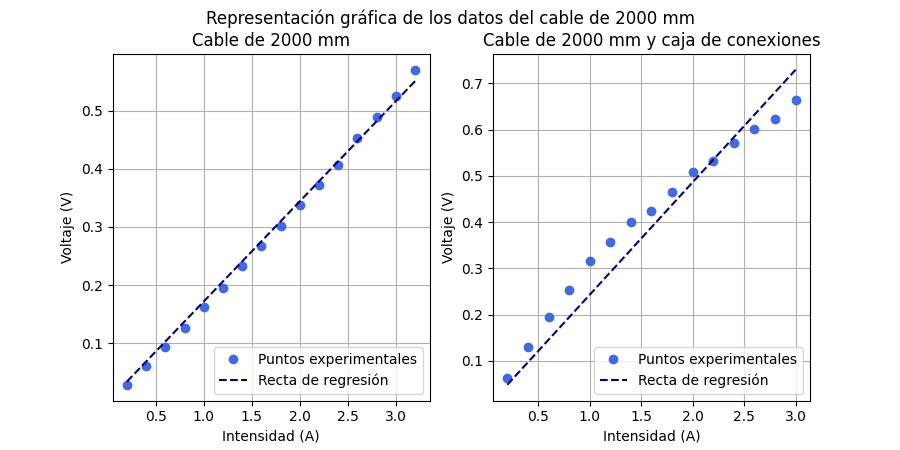
\includegraphics[width=0.95\linewidth]{Images/plotCable3.png}
    \caption{Datos experimentales y rectas de rgresión del cable de 2000 mm}
\end{figure}

\newpage

A partir de los ajustes podemos calcular la resistencia entre contactos de la caja de conexiones y su incertidumbre usando la Ec.\ref{Resistencia contactos} y la Ec.\ref{Inc Resistencia caja}:

\begin{equation}
    \begin{gathered}
        R_{C3} = 0.0355 \; \Omega\\
        s(R_{C3}) = 0.0047\; \Omega
    \end{gathered}
\end{equation}




\newpage

\section{Conclusiones}

Finalmente, vamos a hacer una recapitulación de todos los resultados obtenidos, para poder realizar un análisis global de la práctica. La primera parte de la práctica se centró en determinar la resistividad de dos materiales, el cobre y el aluminio, a partir de la determinación de la resistencia de la barra metálica. Los resultados obtenidos, comparados con los reales obtenidos de \textit{The Handbook of Chemistry and Physics} fueron los siguientes:

\begin{table}[h!]
    \centering
    \begin{tabular}{|c|c|c|}
        \hline
        Material & $\rho_E \pm s(\rho_E) \; (\Omega \cdot m)$ & $\rho \; (\Omega \cdot m)$  \\ \hline
        Cobre  & $1,851 \cdot 10^{-8} \pm 7,7 \cdot 10^{-10}$ & $1.678 \cdot 10^{-8}$ \\ \hline
        Aluminio &$2,58 \cdot 10^{-8} \pm 1,0 \cdot 10^{-9}$ & $2.650\cdot 10^{-8}$\\ \hline
    \end{tabular}
    \caption{Resultados obtenidos para las resistividades}
\end{table}

Como podemos ver, los resultados obtenidos se acercan bastante a los valores reales, las diferencias, pese a que no entran dentro del rango de incertidumbre en el caso del cobre, son muy pequeñas, los valores medidos se corresponden bastante con la realidad. Las pequeñas diferencias las podemos atribuír a los problemas sufridos toda la práctica con los materiales, sobre todo con la fuente de alimentación. Por tanto, podemos concluir que esta primera parte de la práctica fue un éxito.

\par Por otro lado, la segunda parte de la práctica se centró en determinar la resistencia entre contactos de la caja de conexiones. Para ello medimos las diferencias en la resistencia medida solo con el cable y con el cable y la caja de conexiones para tres cables de longitudes diferentes. Los resultados obtenidos de la resistencia entre contactos fueron:

\begin{table}[h!]
    \centering
    \begin{tabular}{|c|c|}
        \hline
        Cable & $R_{C} \pm s(R_C) \; (\Omega)$ \\ \hline
        $100 \; mm$ & $0,006230 \pm 0,000015$\\ \hline
        $600 \; mm$ & $0,017422 \pm 0,000026$\\ \hline
        $2000 \; mm$ & $0,0355 \pm 0,0047$\\ \hline
    \end{tabular}
    \caption{Resultados obtenidos para la resistencia entre contactos}
\end{table}

En esta parte de la práctica los resultados obtenidos difieren bastante más entre sí, llegando las diferencias incluso a un orden de magnitud entre la medida con el primer cable y las otras dos. No obstante, en esta parte de la práctica era hasta cierto punto esperable obtener esas diferencias, sobre todo al trabajar con los cables más largos. Este error sistemático se puede explicar porque las resistencias de los cables con los que trabajamos son notablemente mayores que la resistencia entre contactos de la caja de conexiones, por lo que cualquier falta de precisión en la medida de la resistencia de los cables puede provocar variaciones muy grandes en el valor obtenido de la resistencia entre contactos.

\par Además de eso, otra posible causa para esas diferencias es el mal funcionamiento del material empleado. Como ya hemos explicado anteriormente, al trabajar con intensidades altas en los cables más largos (Por encima de 3 A) los valores de voltaje medidos perdían la linealidad y la fiabilidad. Debido a esto tomamos menos medidas que en el primer cable y las medidas que tomamos probablemente no se ajustarán del todo a los valores reales.

\par Finalmente, pese a todo podemos considerar que hemos alcanzado los objetivos propuestos en la práctica. Conseguimos determinar la resistividad del cobre y del aluminio, obteniendo valores fiables, y conseguimos determinar la resistencia entre contactos de la caja de conexiones, teniendo en cuenta el error sistemático comentado. Además de eso adquirimos una gran experiencia en el manejo de aparatos eléctricos, como la fuente de alimentación, los multímetros y el amplificador.

\section{Bibliografía}

\begin{itemize}
    \item Guión y vídeo explicativo de la práctica de pequeñas resistencias. Campus virtual USC, técnicas experimentales I.
    \item \textit{The Handbook of Chemistry and Physics}
    \item \url{https://es.wikipedia.org/wiki/Ley_de_Ohm}
\end{itemize}

\end{document}